\begin{activity}\label{A:0.5.1}
    Figure \ref{fig:0.5.A1} gives us the voltage produced by an electrical circuit as a function of time.
    \begin{figure}[ht!]
    \begin{center}
        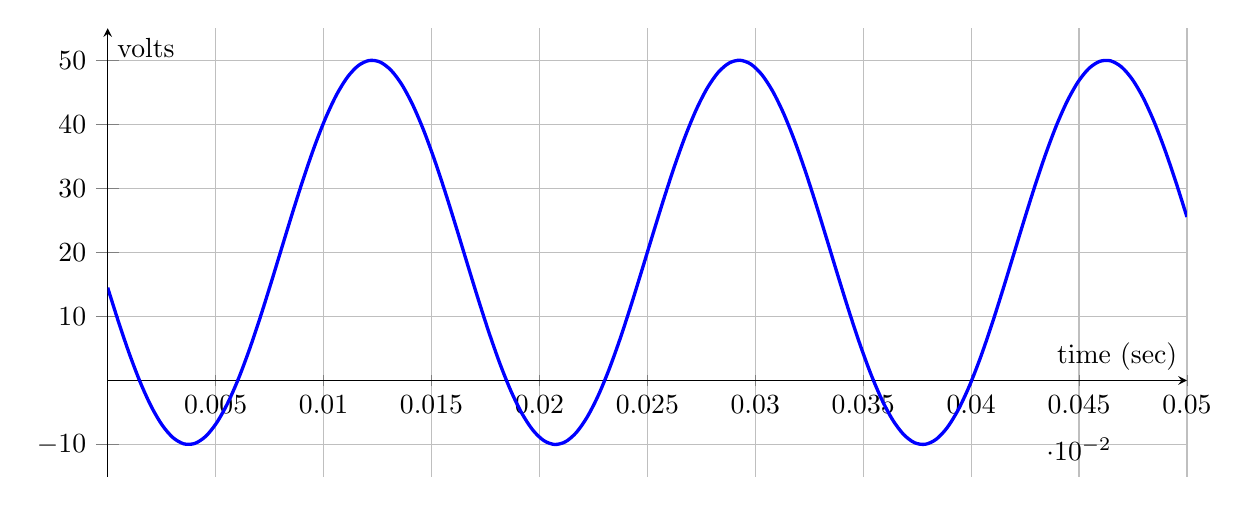
\begin{tikzpicture}
            \begin{axis}[axis lines=center, xmin=0, xmax=0.05, ymin=-15, ymax=55, grid,
                    domain=0:0.05, xlabel={time (sec)}, ylabel={volts},
                    xtick={0.005,0.01,0.015,0.02,0.025,0.03,0.035,0.04,0.045,0.05},
                    xticklabels={0.005,0.01,0.015,0.02,0.025,0.03,0.035,0.04,0.045,0.05},
                ytick={-10,10,20,30,40,50}, xscale=2]
                \addplot[smooth, very thick, blue, samples=100]
                {30*sin(deg(2*pi/0.017*(x-0.008)))+20};
            \end{axis}
        \end{tikzpicture}
    \end{center}
    \caption{Voltage as a function of time.}
    \label{fig:0.5.A1}
\end{figure}
% \resizebox{5in}{!}{\includegraphics{0-5-TrigonometricFunctions5.jpg}}


\ba
\item What is the amplitude of the oscillations?  % 30 volts
\item What is the period of the oscillations? % about 0.017 seconds
\item What is the average value of the voltage?  % 20 volts
\item What is the shift along the $t$ axis, $t_0$?  % about 0.008 seconds
\item What is a formula for this function?  %  V(t) = 30 \sin( 2\pi / 0.017 ( t - 0.008) ) + 20
\ea

\end{activity}\aftera
